\documentclass[a4paper]{jpconf}
\usepackage{graphicx}
\begin{document}
\title{Development of Si Beam Position Detectors for NA61/SHINE experiment}

\author{A. Makhnev$^1$$^,$$^2$, F. Guber$^1$$^,$$^2$, D. Serebryakov$^1$, S. Pulawski$^3$, S. Kowalski$^3$}

\address{$^1$Institute for Nuclear Research RAS, Moscow, Russia}
\address{$^2$Moscow Institute of Physics and Technology, Dolgoprudny, Moscow Region, Russia}
\address{$^3$Institute of Physics, University of Silesia, Chorzów, Poland}

\ead{makhnev.a@phystech.edu}

\begin{abstract}
The NA61/SHINE detector at the CERN SPS is undergoing a major upgrade during the LHC Long Shutdown 2 period (2019-2021). The upgrade is essential to fulfil the requirements of the new open charm measurement program. In this program detector will operate at a beam intensity increased by a factor of 10, which requires an upgrade of current Beam Position Detectors (BPDs). New BPDs should monitor lead and proton beam intensities with 10$^5$ Hz intensity. In this article, progress on design and development of the new BPDs based on Si strip detectors, its front-end and readout electronics, as well as integration with the NA61/SHINE DAQ will be presented.
\end{abstract}

\section{Introduction}

NA61/SHINE is a fixed-target experiment located in the H2 line in the North Area of the CERN Super Proton Synchrotron (SPS)~\cite{Abgrall:2014fa}. The multi-purpose detector is optimized to study hadron production in hadron-proton, hadron-nucleus and nucleus-nucleus collisions. Figure~\ref{fig:1} presents a schematic drawing of the detector after the Long Shutdown 2 (LS2) upgrades. It consists of a large acceptance hadron spectrometer with excellent capabilities in charged particle momentum measurements and identification by a set of eight Time Projection Chambers (TPC) as well as Time-of-Flight (ToF) detectors. The Vertex Detector (SAVD) is placed 5~cm centimetres downstream from the target. It consists of four layers of silicon pixel sensors allowing to reconstruct vertices of short-lived charm particles like D$^0$ mesons. The high resolution forward calorimeter, the Projectile Spectator Detector (PSD), measures energy flow around the beam direction, which in nucleus-nucleus reactions is primarily a measure of the number of spectator (non-interacting) nucleons. An array of beam detectors identifies beam particles, secondary hadrons and ions as well as primary ions, and measures precisely their trajectories.

\begin{figure}[htbp]
	\centering
	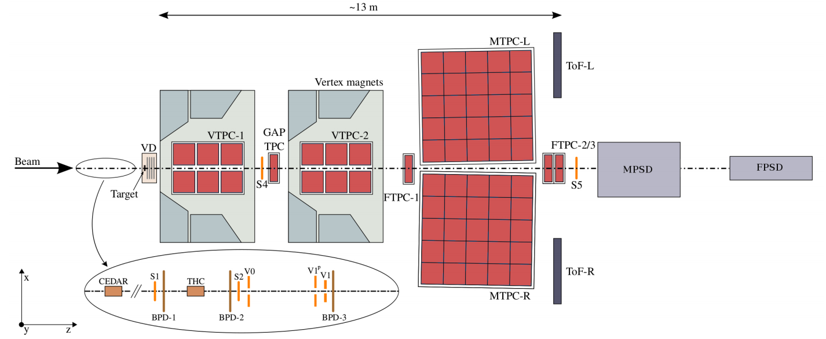
\includegraphics[width=\textwidth]{NA61_scheme.png}
	\caption{\label{fig:1} NA61/SHINE experiment after the LS2 upgrades}
\end{figure}

\section{New BPD requirements}
The main purpose of BPDs detectors is measurement of beam particle trajectory on event-by-event basis (particle-by-particle). New BPDs should monitor lead and proton beam intensities with 10$^5$Hz intensity and should operate in vacuum, which renders previous solutions (proportional chambers non-feasible). Other detector requirements include:
\begin{enumerate}
	\item Detector/detectors should work with p and Pb beams
	\item The planed beam intensity is on the level of 100~kHz of Pb or p ions at momentum 13-150 $AGeV/c$.
	\item For this purpose detector should be able to determine without doubts the position of X and Y hit of each beam particle (probability of pileup should be minimised).
	\item The accuracy of the position measurement is expected to be on the level of 250~$\mu$m.
	\item Detector should be installed in the vacuum $\left(10^{-6}\right)$.
	\item Material on the beam line should be minimised.
\end{enumerate}

\section{New BPD design}

\subsection{Detector position on the beam line}
On NA61/SHINE beam profile is measured by a telescope consisting out of 3 separate detectors with 2-coordinate determination of the beam particle position. These 3 detectors are mounted before the target.

\subsection{Sensitive element selection}
In this work, only the design of Silicon Strip Detector (SSD) version of the BPDs will be presented, although design based on the scintillating fibres has also been considered.
In order to fulfil above-mentioned requirements, a Hamamatsu S13804 detector has been chosen, meeting constraints on accuracy and sensitivity.
For this application, SSDs have a set of advantages, including: being an off-the-shelf component and having a sufficient radiation hardness for this application. Such detectors have been already used for similar task at BM@N, LHC, J-PARC and other experiments.

\subsection{Mechanical design}
Each of the 3 BPDs will utilize a 6-way vacuum fitting with 2 of the openings being connected to the beam pipe, 2 having the detector inserts mounted to them and 2 being plugged. (see figure~\ref{fig:2}).

\begin{figure}[htbp]
	\centering
	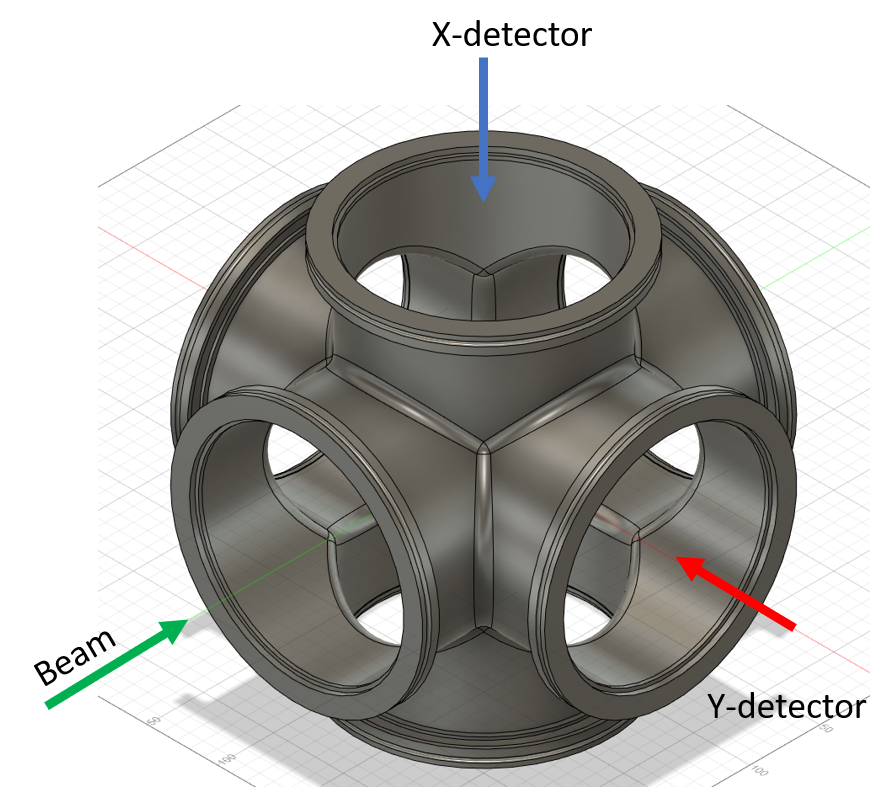
\includegraphics[width=.5\textwidth]{6_way_fitting.png}
	\caption{\label{fig:2} 6-way vacuum fitting}
\end{figure}

Each of the detector inserts consists out of an ISO-K vacuum flange with a seal/centering ring, with two vacuum feedthrough connectors and two optical mounting brackets machined into it. An aluminium plate with an opening for the beam is mounted onto the brackets to ensure precise positioning of the detector in the beam pipe. A flexible PCB is then mounted onto the aluminium plate, which hosts the detector itself and two mating connectors for the feedthrough. Usage of flexible PCB ensure minimum gas emission and removes the need for additional connectors between the detector and the front-end amplifiers. Design is presented on the figure~\ref{fig:3} and ~\ref{fig:4}.

\begin{figure}[htbp]
	\begin{minipage}{14pc}
		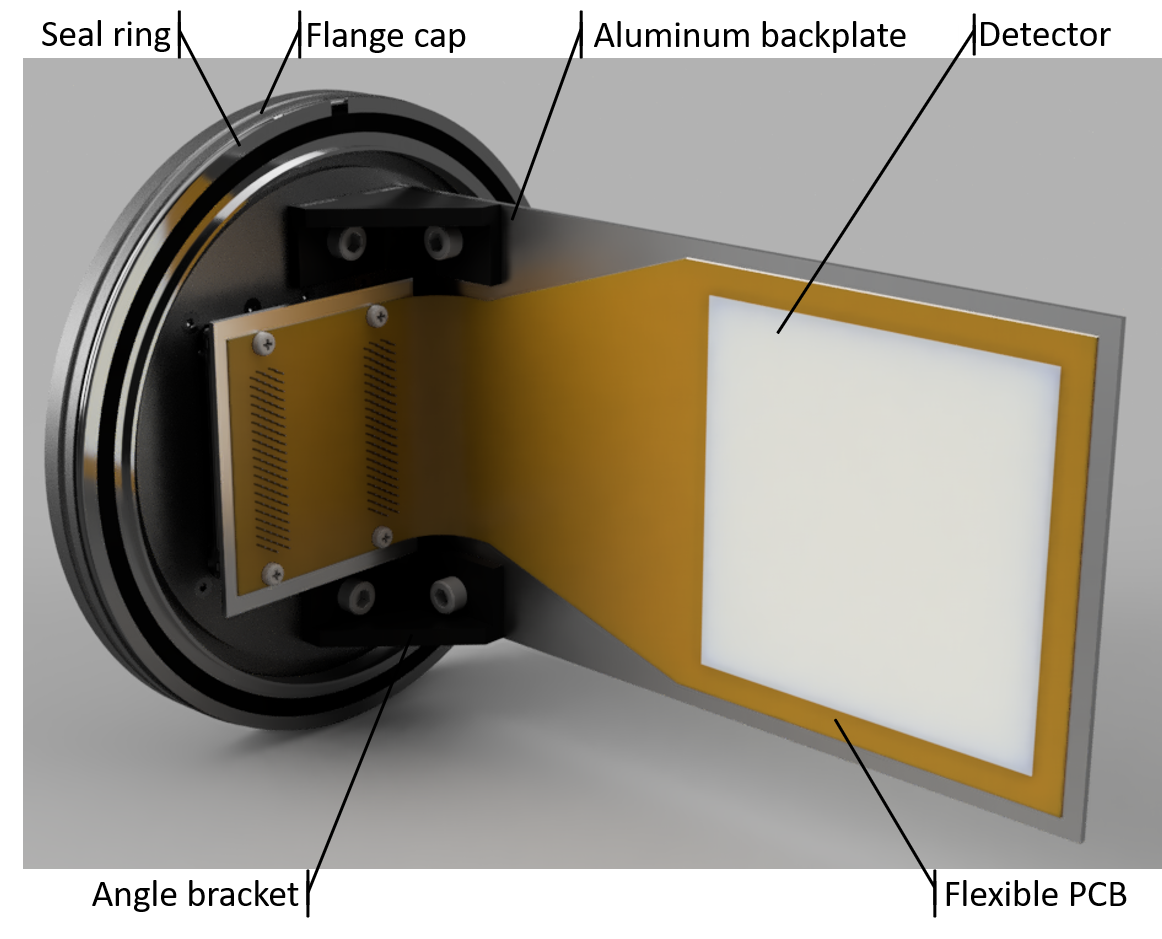
\includegraphics[width=\textwidth]{detector_insert.png}
		\caption{\label{fig:3} Detector insert, overall view}
	\end{minipage}\hspace{2pc}
	\begin{minipage}{14pc}
		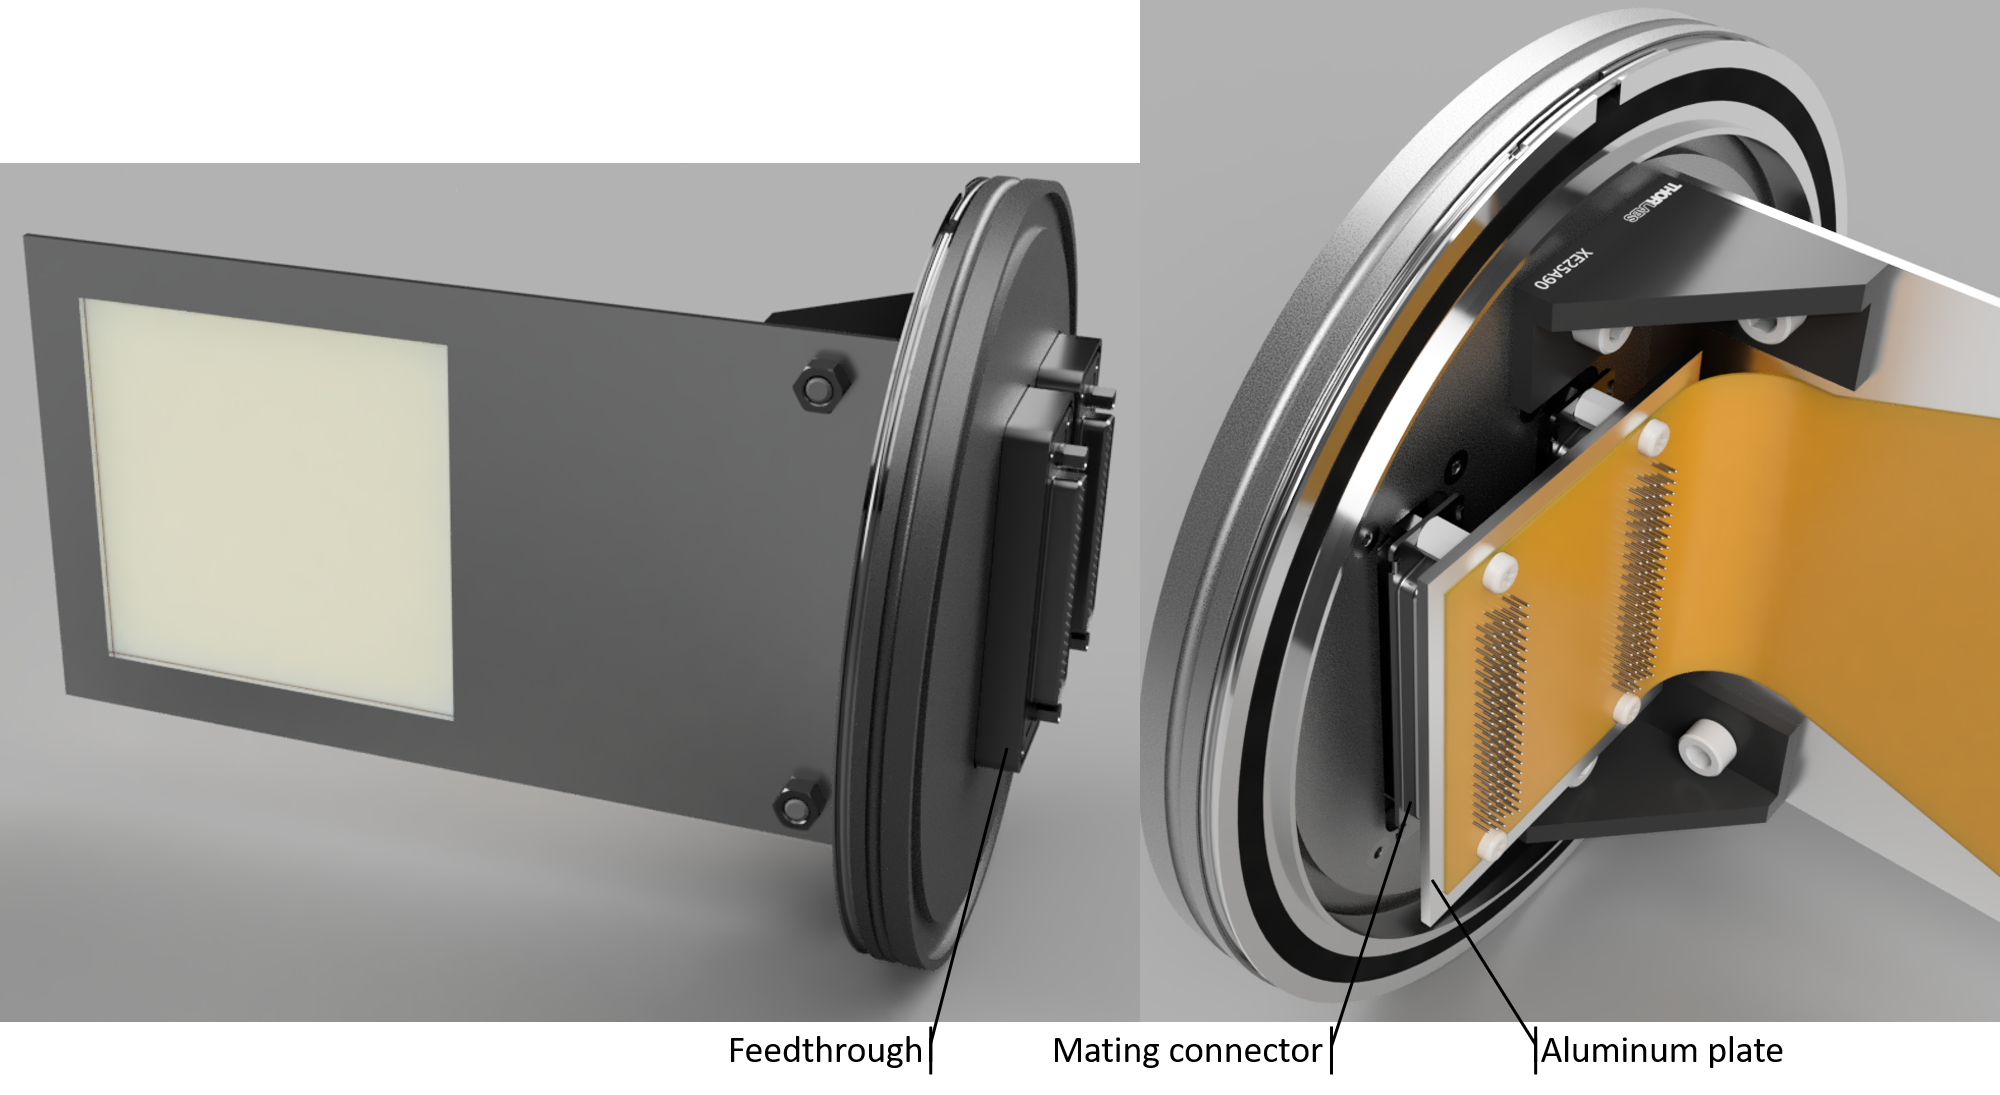
\includegraphics[width=1.5\textwidth]{detector_insert_back.png}
		\caption{\label{fig:4} Detector insert, detailed view}
	\end{minipage} 
\end{figure}

Mounting fixtures are offset, so the beam would hit the middle of the sensitive part of the detector, as the topology illustrations show that the sensitive elements are arranged as two columns with bonding pads in the middle, see figures ~\ref{fig:5} and ~\ref{fig:6}.

\begin{figure}[htbp]
	\begin{minipage}{18pc}
		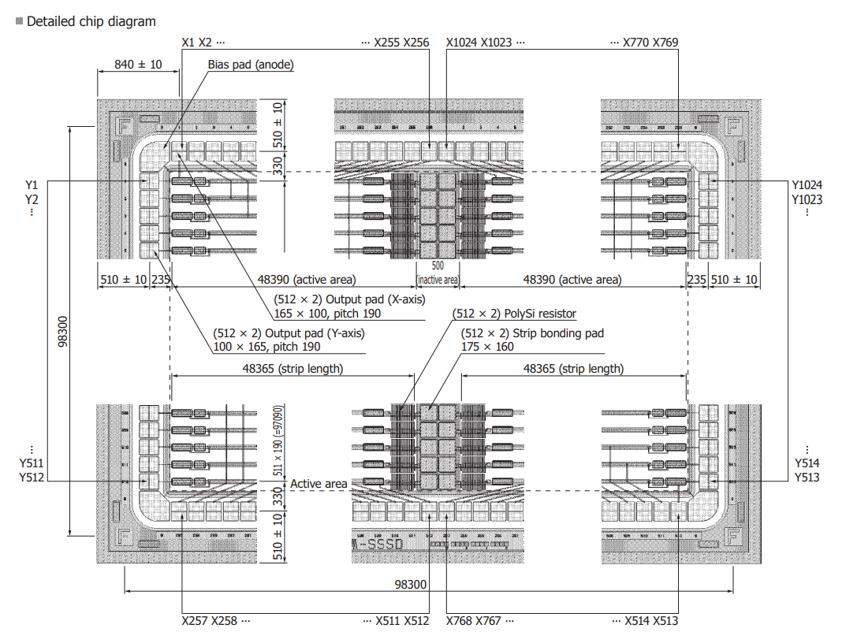
\includegraphics[width=\textwidth]{topology.png}
		\caption{\label{fig:5} Detector topology view}
	\end{minipage}\hspace{2pc}
	\begin{minipage}{13pc}
		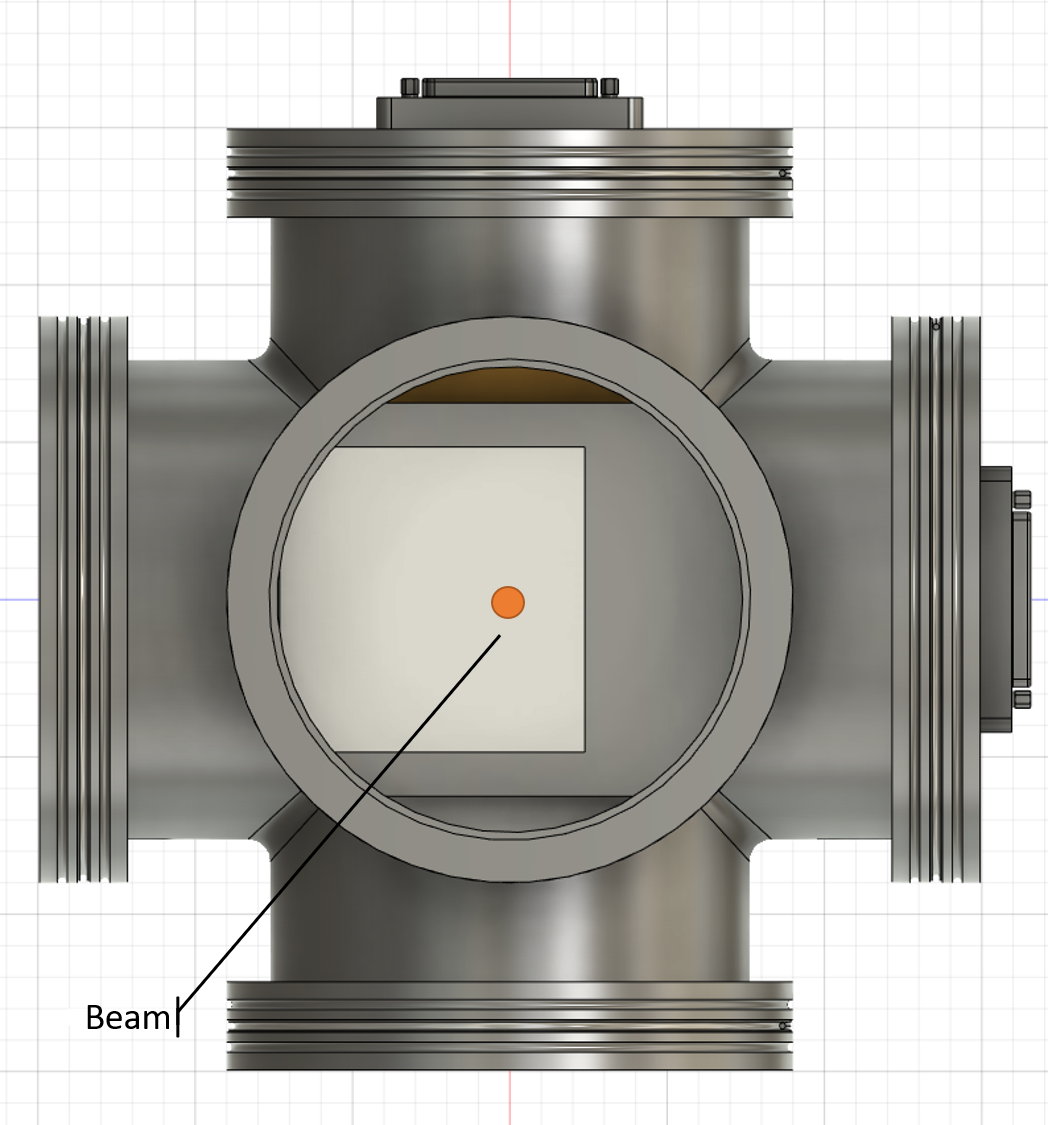
\includegraphics[width=\textwidth]{fixture_offset.png}
		\caption{\label{fig:6} Mounting fixture design}
	\end{minipage} 
\end{figure}

\section{Front End Electronics design}
A design of typical front end electronics has been developed. Schematic is built entirely out of off-the-shelf components, without usage of any custom-manufactured ASICs or other expensive or hard to obtain parts.

Typical amplifier consists out of fast and charge-sensitive amplifier, an intermediate amplifier and an output buffer (see figures ~\ref{fig:7} and ~\ref{fig:8}). An electronically-controlled scale-changing feature has been added later, making the same board usable with both proton and heavy ion beams.

An evaluation board with one typical amplifier has been manufactured (see figure ~\ref{fig:8}) and tested for amplification and noise spectrum with satisfactory results (see figure ~\ref{fig:9} and ~\ref{fig:10}).

\begin{figure}[htbp]
	\begin{minipage}{18pc}
		\includegraphics[width=\textwidth]{schematic.png}
		\caption{\label{fig:7} Typical amplifier schematic}
	\end{minipage}\hspace{2pc}
	\begin{minipage}{18pc}
		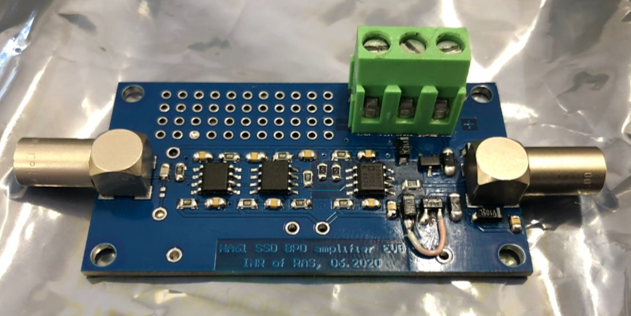
\includegraphics[width=\textwidth]{amp_photo.png}
		\caption{\label{fig:8} Evaluation board}
	\end{minipage} 
\end{figure}

\begin{figure}[htbp]
	\begin{minipage}{18pc}
		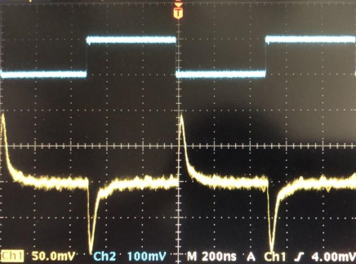
\includegraphics[width=\textwidth]{osc.png}
		\caption{\label{fig:9} Amplifier output signal with generator input}
	\end{minipage}\hspace{2pc}
	\begin{minipage}{18pc}
		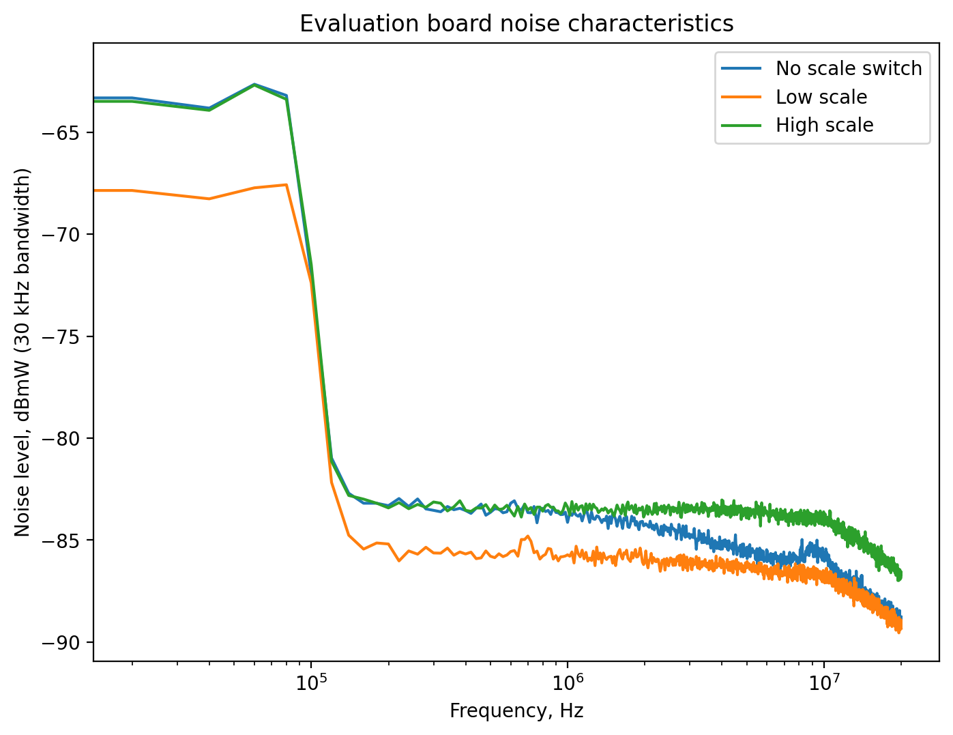
\includegraphics[width=\textwidth]{noise.png}
		\caption{\label{fig:10} Noise characteristics}
	\end{minipage} 
\end{figure}


\end{document}


